\documentclass[11pt]{standalone}

\usepackage{units}
\usepackage{ifthen}
\usepackage{tikz} 
\usetikzlibrary{shapes.misc}
\usetikzlibrary{arrows,arrows.meta}
\usetikzlibrary{calc,intersections, patterns, math}

\definecolor{pfeil}{RGB}{168,167,167}
\definecolor{petrol}{RGB}{0, 118, 136}
\definecolor{darkgoldenrod}{RGB}{184, 134, 11}
\colorlet{petrol-lighter}{petrol!40}
\colorlet{darkgoldenrod-lighter}{darkgoldenrod!40}

\begin{document}

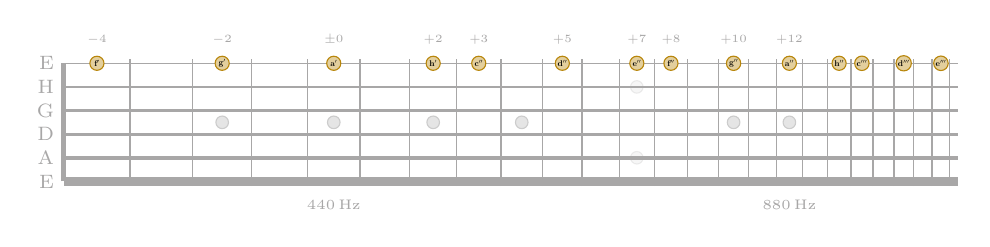
\begin{tikzpicture}[pfeil,
    ynode/.style={draw=darkgoldenrod,circle,fill=darkgoldenrod-lighter,scale=.3,inner sep=1pt,minimum size=1.7em}]

  %%%% Draw the base and set coordinates %%%%
  \begin{scope}[xscale=-15,yscale=.3,line width=.5]

    \xdef\x{1}
    %% Left line
    \draw[line width=1.75] (1,1) -- (1,6);
    \foreach \fret in {1,...,24}{
      %% Set coordinate for each string
      \foreach \str in {0,...,6}{
        \coordinate (\str-\fret) at (0.97193715634*\x,\str);
      }
      %% Set coordinate for the text above
      \coordinate (Top-\fret) at (0.97193715634*\x,7);
      %% Compute the position of the fret
      \pgfmathsetmacro\x{\x * 0.94387431268}
      \xdef\x{\x}
      %% Draw the fret
      \draw (\x,0.8) -- (\x,6.2);
    }

    %% Draw each string
    \foreach \str in {1,...,6}{
      \draw[line width=3/\str] (1,\str) -- (0.97153194115*\x,\str);
      \coordinate (start\str) at (1,\str);
    }
  \end{scope}

  %% Draw the mark on the guitare
  \foreach \f in {3,5,7,9,15,17}{
    \draw[black!20,fill=black!10] ($(3-\f)!.5!(4-\f)$) circle (.08);
  }
  \draw[opacity=.20,fill,fill opacity=.10] (2-12) circle (.08) (5-12) circle (.08);

  %% We define the name of each number
  \newcommand\savename[2]{\expandafter\xdef\csname name#1\endcsname{#2}}
%   \newcommand\getname[1]{\csname name#1\endcsname}
%   \foreach \n/\t in {1/a,2/,3/h,4/c,5/,6/d,7/,8/e,9/f,10/,11/g,0/}{
%     \savename{\n}{\t}
%   }
  \newcommand\getNames[1]{\csname name#1\endcsname}
  \foreach \n/\t in {1/A,2/,3/H,4/C,5/,6/D,7/,8/E,9/F,10/,11/G,0/}{
    \savename{\n}{\t}
  }

  %% Boucle on the string and the first note (given its number)
  \foreach \str/\note in {1/8,2/1,3/6,4/11,5/3,6/8}{
    \node[anchor=east] at (start\str) {\scriptsize\getNames{\note}};

    % \foreach \fret in {1,...,24}{
    %   \pgfmathtruncatemacro\note{mod( \note+1, 12 )}
    %   \xdef\note{\note}
    %   \node[ynode] at (6-\fret) {\textbf{\getname{\note}}};
    % }
  }

  \newcommand\getname[1]{\csname name#1\endcsname}
  \foreach \n/\t in {1/a,2/,3/h,4/c,5/,6/d,7/,8/e,9/f,10/,11/g,0/}{
    \savename{\n}{\t}
  }

    \node[ynode] at (6-1) {\textbf{\color{black}\getname{9}$'$}};
    \node[ynode] at (6-3) {\textbf{\color{black}\getname{11}$'$}};
    \node[ynode] at (6-5) {\textbf{\color{black}\getname{1}$'$}};
    \node[ynode] at (6-7) {\textbf{\color{black}\getname{3}$'$}};
    \node[ynode] at (6-8) {\textbf{\color{black}\getname{4}$''$}};
    \node[ynode] at (6-10) {\textbf{\color{black}\getname{6}$''$}};
    \node[ynode] at (6-12) {\textbf{\color{black}\getname{8}$''$}};
    \node[ynode] at (6-13) {\textbf{\color{black}\getname{9}$''$}};
    \node[ynode] at (6-15) {\textbf{\color{black}\getname{11}$''$}};
    \node[ynode] at (6-17) {\textbf{\color{black}\getname{1}$''$}};
    \node[ynode] at (6-19) {\textbf{\color{black}\getname{3}$''$}};
    \node[ynode] at (6-20) {\textbf{\color{black}\getname{4}$'''$}};
    \node[ynode] at (6-22) {\textbf{\color{black}\getname{6}$'''$}};
    \node[ynode] at (6-24) {\textbf{\color{black}\getname{8}$'''$}};

    \node[] at (0-5) {$\scriptscriptstyle\unit[440]{Hz}$};
    \node[] at (0-17) {$\scriptscriptstyle\unit[880]{Hz}$};

  %% Number above each space
  \foreach \fret in {1,3}{
    \pgfmathtruncatemacro\nummer{\fret-5}
    \node[scale=.8] at (Top-\fret) {\tiny $\nummer$};
  }
  \foreach \fret in {5}{
    \pgfmathtruncatemacro\nummer{\fret-5}
    \node[scale=.8] at (Top-\fret) {\tiny $\pm\nummer$};
  }
  \foreach \fret in {7,8,10,12,13,15,17}{
    \pgfmathtruncatemacro\nummer{\fret-5}
    \node[scale=.8] at (Top-\fret) {\tiny $+\nummer$};
  }


\end{tikzpicture}

\end{document}
